\section{Tabellen}
\label{sec:Tabellen}
\begin{table}[H]
  \centering
  \caption{Umgerechnete Messwerte der 1.Messung $(b_\text{heiz} = \SI{1.5}{\kelvin\per\minute})$}
  \label{tab:1}
    \begin{tabular}{S S S S S S}
    \toprule
    $\text{i(T)} \: / \: \num{10e-11} \, \si{\ampere} $ & $ T \: / \: \si{\kelvin}$
    & $ t \: / \: \si{\second}$ &
    $\text{i(T)} \: / \: \num{10e-11} \, \si{\ampere} $ & $ T \: / \: \si{\kelvin}$
    & $ t \: / \: \si{\second}$\\
    \midrule
    0.000 & 211.55 & 0 & 0.390 & 275.15 & 2520 \\
    0.000 & 213.95 & 60 & 0.410 & 276.75 & 2580 \\
    0.012 & 215.65 & 120 & 0.420 & 278.25 & 2640 \\
    0.024 & 217.65 & 180 & 0.440 & 279.55 & 2700 \\
    0.042 & 219.45 & 240 & 0.460 & 280.95 & 2760 \\
    0.096 & 220.85 & 300 & 0.480 & 282.35 & 2820 \\
    0.102 & 222.35 & 360 & 0.500 & 283.65 & 2880 \\
    0.105 & 223.75 & 420 & 0.520 & 285.05 & 2940 \\
    0.108 & 225.45 & 480 & 0.550 & 286.55 & 3000 \\
    0.108 & 227.25 & 540 & 0.570 & 288.05 & 3060 \\
    0.117 & 228.75 & 600 & 0.590 & 289.45 & 3120 \\
    0.123 & 229.85 & 660 & 0.610 & 290.85 & 3180 \\
    0.129 & 231.35 & 720 & 0.620 & 292.15 & 3240 \\
    0.138 & 232.95 & 780 & 0.640 & 293.65 & 3300 \\
    0.156 & 234.75 & 840 & 0.660 & 295.15 & 3360 \\
    0.180 & 236.65 & 900 & 0.680 & 296.65 & 3420 \\
    0.207 & 238.25 & 960 & 0.690 & 297.95 & 3480 \\
    0.234 & 239.45 & 1020 & 0.710 & 299.45 & 3540 \\
    0.270 & 240.85 & 1080 & 0.740 & 300.95 & 3600 \\
    0.300 & 242.15 & 1140 & 0.780 & 302.45 & 3660 \\
    0.360 & 243.45 & 1200 & 0.800 & 303.95 & 3720 \\
    0.440 & 244.95 & 1260 & 0.870 & 305.35 & 3780 \\
    0.510 & 246.65 & 1320 & 0.920 & 306.85 & 3840 \\
    0.620 & 248.05 & 1380 & 0.990 & 308.25 & 3900 \\
    0.740 & 249.55 & 1440 & 1.050 & 309.85 & 3960 \\
    0.870 & 251.05 & 1500 & 1.110 & 311.35 & 4020 \\
    1.000 & 252.55 & 1560 & 1.200 & 312.95 & 4080 \\
    1.170 & 254.05 & 1620 & 1.260 & 314.55 & 4140 \\
    1.260 & 255.55 & 1680 & 1.350 & 316.15 & 4200 \\
    1.350 & 256.95 & 1740 & 1.380 & 317.75 & 4260 \\
    1.410 & 258.35 & 1800 & 1.380 & 319.25 & 4320 \\
    1.410 & 259.75 & 1860 & 1.380 & 320.75 & 4380 \\
    1.350 & 261.15 & 1920 & 1.320 & 322.25 & 4440 \\
    1.260 & 262.75 & 1980 & 1.260 & 323.75 & 4500 \\
    1.080 & 264.25 & 2040 & 1.200 & 325.35 & 4560 \\
    0.930 & 265.65 & 2100 & 1.110 & 326.65 & 4620 \\
    0.750 & 267.05 & 2160 & 1.020 & 327.95 & 4680 \\
    0.600 & 268.45 & 2220 & 0.930 & 329.95 & 4740 \\
    0.500 & 269.95 & 2280 & 0.870 & 331.15 & 4800 \\
    0.430 & 271.35 & 2340 & 0.760 & 332.75 & 4860 \\
    0.400 & 272.65 & 2400 & 0.740 & 333.15 & 4875 \\
    0.390 & 273.95 & 2460 &       &        &      \\
    \bottomrule
  \end{tabular}
\end{table}

\begin{table}[H]
  \centering
  \caption{Umgerechnete Messwerte der 2.Messung $(b_\text{heiz} =
  \SI{3.0}{\kelvin\per\minute})$}
  \label{tab:2}
    \begin{tabular}{S S S}
    \toprule
    $ \text{i(T)}  \: / \: 10^{-11} \, \si{\ampere} $ & $ T\: / \: \si{\kelvin} $
    & $ t \: / \: \si{\second} $ \\
    \midrule
    0.000 & 213.25 & 0 \\
    0.114 & 214.85 & 60 \\
    0.114 & 216.75 & 12 \\
    0.117 & 219.25 & 180 \\
    0.126 & 222.25 & 240 \\
    0.135 & 225.25 & 300 \\
    0.147 & 228.25 & 360 \\
    0.165 & 231.35 & 420 \\
    0.189 & 234.45 & 480 \\
    0.225 & 237.45 & 540 \\
    0.290 & 240.55 & 600 \\
    0.360 & 243.35 & 660 \\
    0.510 & 246.15 & 720 \\
    0.700 & 248.95 & 780 \\
    0.980 & 251.65 & 840 \\
    1.380 & 254.55 & 900 \\
    1.920 & 257.65 & 960 \\
    2.430 & 260.75 & 1020 \\
    2.760 & 263.75 & 1080 \\
    2.640 & 266.95 & 1140 \\
    2.130 & 269.85 & 1200 \\
    1.440 & 272.65 & 1260 \\
    0.900 & 275.25 & 1320 \\
    0.780 & 277.95 & 1380 \\
    0.750 & 280.65 & 1440 \\
    0.760 & 283.45 & 1500 \\
    0.820 & 286.35 & 1560 \\
    0.910 & 289.25 & 1620 \\
    0.950 & 292.05 & 1680 \\
    1.020 & 294.75 & 1740 \\
    1.050 & 297.65 & 1800 \\
    1.080 & 300.55 & 1860 \\
    1.110 & 303.55 & 1920 \\
    1.200 & 306.55 & 1980 \\
    1.380 & 309.65 & 2040 \\
    1.590 & 312.55 & 2100 \\
    1.740 & 315.45 & 2160 \\
    1.920 & 318.35 & 2220 \\
    2.040 & 321.15 & 2280 \\
    2.040 & 323.95 & 2340 \\
    1.860 & 326.85 & 2400 \\
    1.620 & 329.65 & 2460 \\
    \bottomrule
  \end{tabular}
\end{table}

\begin{table}[H]
  \centering
  \caption{Werte des Integrals von $i(T)$ der 1.Messung $(b_\text{heiz} =
  \SI{1.5}{\kelvin\per\minute})$}
  \label{tab:3}
    \begin{tabular}{S S S S}
    \toprule
    $ T \: / \: \si{\kelvin} $ & $ \text{Integral von  i(T)} \: / \:
    \num{10e-11} \, \si{\ampere}$ & $ \text{Integral von } \Delta \text{i(T)} \: / \:
    \num{10e-11} \, \si{\ampere}$ &
    $ \text{i(T)}  \: / \:  10^{-11} \, \si{\ampere} $ \\
    \midrule
    269.950 & 0.071 & 0.079 & 0.500 \\
    268.450 & 0.289 & 0.163 & 0.600 \\
    267.050 & 0.681 & 0.242 & 0.750 \\
    265.650 & 1.318 & 0.321 & 0.930 \\
    264.250 & 2.199 & 0.399 & 1.080 \\
    262.750 & 3.406 & 0.484 & 1.260 \\
    261.150 & 4.926 & 0.574 & 1.350 \\
    259.750 & 6.376 & 0.653 & 1.410 \\
    258.350 & 7.881 & 0.731 & 1.410 \\
    256.950 & 9.357 & 0.810 & 1.350 \\
    255.550 & 10.742 & 0.889 & 1.260 \\
    254.050 & 12.106 & 0.973 & 1.170 \\
    252.550 & 13.290 & 1.058 & 1.000 \\
    251.050 & 14.264 & 1.142 & 0.870 \\
    249.550 & 15.059 & 1.226 & 0.740 \\
    248.050 & 15.682 & 1.311 & 0.620 \\
    246.650 & 16.117 & 1.389 & 0.510 \\
    244.950 & 16.509 & 1.485 & 0.440 \\
    243.450 & 16.760 & 1.569 & 0.360 \\
    242.150 & 16.898 & 1.643 & 0.300 \\
    240.850 & 16.989 & 1.716 & 0.270 \\
    239.450 & 17.055 & 1.794 & 0.234 \\
    238.250 & 17.084 & 1.862 & 0.207 \\
    236.650 & 17.094 & 1.952 & 0.180 \\
    234.750 & 17.081 & 2.059 & 0.156 \\
    232.950 & 17.054 & 2.160 & 0.138 \\
    231.350 & 17.027 & 2.250 & 0.129 \\
    229.850 & 17.006 & 2.334 & 0.123 \\
    228.750 & 16.994 & 2.396 & 0.117 \\
    227.250 & 16.980 & 2.481 & 0.108 \\
    225.450 & 16.975 & 2.582 & 0.108 \\
    223.750 & 16.988 & 2.678 & 0.105 \\
    222.350 & 17.010 & 2.756 & 0.102 \\
    220.850 & 17.041 & 2.841 & 0.096 \\
    219.450 & 17.042 & 2.919 & 0.042 \\
    217.650 & 16.999 & 3.021 & 0.024 \\
    215.650 & 16.946 & 3.133 & 0.012 \\
    \bottomrule
  \end{tabular}
\end{table}

\begin{table}[H]
  \centering
  \caption{Werte des Integrals von $i(T)$ der 1.Messung $(b_\text{heiz} =
  \SI{3.0}{\kelvin\per\minute})$}
  \label{tab:4}
    \begin{tabular}{S S S S}
    \toprule
    $ T\: / \: \si{\kelvin} $ & $ \text{Integral von  i(T)} \: / \:
    \num{10e-11} \, \si{\ampere}$ & $ \text{Integral von } \Delta \text{i(T)} \: / \:
    \num{10e-11} \, \si{\ampere}$ &
    $ \text{i(T)}  \: / \:  \num{10e-11} \, \si{\ampere} $ \\
    \midrule
    275.250 & 0.317 & 0.283 & 0.900 \\
    272.650 & 1.561 & 0.555 & 1.440 \\
    269.850 & 4.709 & 0.849 & 2.130 \\
    266.950 & 9.806 & 1.153 & 2.640 \\
    263.750 & 16.552 & 1.488 & 2.760 \\
    260.750 & 22.669 & 1.803 & 2.430 \\
    257.650 & 27.797 & 2.127 & 1.920 \\
    254.550 & 31.409 & 2.452 & 1.380 \\
    251.650 & 33.526 & 2.756 & 0.980 \\
    248.950 & 34.667 & 3.039 & 0.700 \\
    246.150 & 35.281 & 3.333 & 0.510 \\
    243.350 & 35.511 & 3.626 & 0.360 \\
    240.550 & 35.523 & 3.920 & 0.290 \\
    237.450 & 35.433 & 4.244 & 0.225 \\
    234.450 & 35.301 & 4.559 & 0.189 \\
    231.350 & 35.181 & 4.884 & 0.165 \\
    228.250 & 35.107 & 5.209 & 0.147 \\
    225.250 & 35.097 & 5.523 & 0.135 \\
    222.250 & 35.160 & 5.837 & 0.126 \\
    \bottomrule
  \end{tabular}
\end{table}

\begin{table}[H]
  \centering
  \caption{Werte für die Aktivierungsenergiebestimmung der 1.Messung
  $(b_\text{heiz} =
  \SI{1.5}{\kelvin\per\minute})$}
  \label{tab:5}
    \begin{tabular}{S S S S}
    \toprule
    $ \text{ln(j)} $ & $ T \: / \:\si{\kelvin}$
    & $ \text{ln(j)} $ & $ T \: / \:\si{\kelvin}$ \\
    \midrule
    -16.747 & 215.65 & -13.265 & 275.15 \\
    -16.054 & 217.65 & -13.215 & 276.75 \\
    -15.494 & 219.45 & -13.191 & 278.25 \\
    -14.667 & 220.85 & -13.145 & 279.55 \\
    -14.607 & 222.35 & -13.100 & 280.95 \\
    -14.578 & 223.75 & -13.058 & 282.35 \\
    -14.549 & 225.45 & -13.017 & 283.65 \\
    -14.549 & 227.25 & -12.978 & 285.05 \\
    -14.469 & 228.75 & -12.922 & 286.55 \\
    -14.419 & 229.85 & -12.886 & 288.05 \\
    -14.372 & 231.35 & -12.851 & 289.45 \\
    -14.304 & 232.95 & -12.818 & 290.85 \\
    -14.182 & 234.75 & -12.802 & 292.15 \\
    -14.039 & 236.65 & -12.770 & 293.65 \\
    -13.899 & 238.25 & -12.739 & 295.15 \\
    -13.776 & 239.45 & -12.710 & 296.65 \\
    -13.633 & 240.85 & -12.695 & 297.95 \\
    -13.528 & 242.15 & -12.666 & 299.45 \\
    -13.346 & 243.45 & -12.625 & 300.95 \\
    -13.145 & 244.95 & -12.572 & 302.45 \\
    -12.997 & 246.65 & -12.547 & 303.95 \\
    -12.802 & 248.05 & -12.463 & 305.35 \\
    -12.625 & 249.55 & -12.407 & 306.85 \\
    -12.463 & 251.05 & -12.334 & 308.25 \\
    -12.324 & 252.55 & -12.275 & 309.85 \\
    -12.167 & 254.05 & -12.219 & 311.35 \\
    -12.093 & 255.55 & -12.142 & 312.95 \\
    -12.024 & 256.95 & -12.093 & 314.55 \\
    -11.980 & 258.35 & -12.024 & 316.15 \\
    -11.980 & 259.75 & -12.002 & 317.75 \\
    -12.024 & 261.15 & -12.002 & 319.25 \\
    -12.093 & 262.75 & -12.002 & 320.75 \\
    -12.247 & 264.25 & -12.046 & 322.25 \\
    -12.396 & 265.65 & -12.093 & 323.75 \\
    -12.612 & 267.05 & -12.142 & 325.35 \\
    -12.835 & 268.45 & -12.219 & 326.65 \\
    -13.017 & 269.95 & -12.304 & 327.95 \\
    -13.168 & 271.35 & -12.396 & 329.95 \\
    -13.240 & 272.65 & -12.463 & 331.15 \\
    -13.265 & 273.95 & -12.598 & 332.75 \\
    \bottomrule
  \end{tabular}
\end{table}

\begin{table}[H]
  \centering
  \caption{Werte für die Aktivierungsenergiebestimmung der 1.Messung
  $(b_\text{heiz} =
  \SI{3.0}{\kelvin\per\minute})$}
  \label{tab:6}
    \begin{tabular}{S S S S}
    \toprule
    $ \text{ln(j)} $ & $ T \: / \:\si{\kelvin}$
    & $ \text{ln(j)} $ & $ T \: / \:\si{\kelvin}$ \\
    \midrule
    -14.495 & 214.85 & -11.959 & 272.65 \\
    -14.495 & 216.75 & -12.429 & 275.25 \\
    -14.469 & 219.25 & -12.572 & 277.95 \\
    -14.395 & 222.25 & -12.612 & 280.65 \\
    -14.326 & 225.25 & -12.598 & 283.45 \\
    -14.241 & 228.25 & -12.522 & 286.35 \\
    -14.126 & 231.35 & -12.418 & 289.25 \\
    -13.990 & 234.45 & -12.375 & 292.05 \\
    -13.816 & 237.45 & -12.304 & 294.75 \\
    -13.562 & 240.55 & -12.275 & 297.65 \\
    -13.346 & 243.35 & -12.247 & 300.55 \\
    -12.997 & 246.15 & -12.219 & 303.55 \\
    -12.681 & 248.95 & -12.142 & 306.55 \\
    -12.344 & 251.65 & -12.002 & 309.65 \\
    -12.002 & 254.55 & -11.860 & 312.55 \\
    -11.672 & 257.65 & -11.770 & 315.45 \\
    -11.436 & 260.75 & -11.672 & 318.35 \\
    -11.309 & 263.75 & -11.611 & 321.15 \\
    -11.353 & 266.95 & -11.611 & 323.95 \\
    -11.568 & 269.85 & -11.703 & 326.85 \\
    \bottomrule
  \end{tabular}
\end{table}
\section{Messwerte}

\begin{figure}
  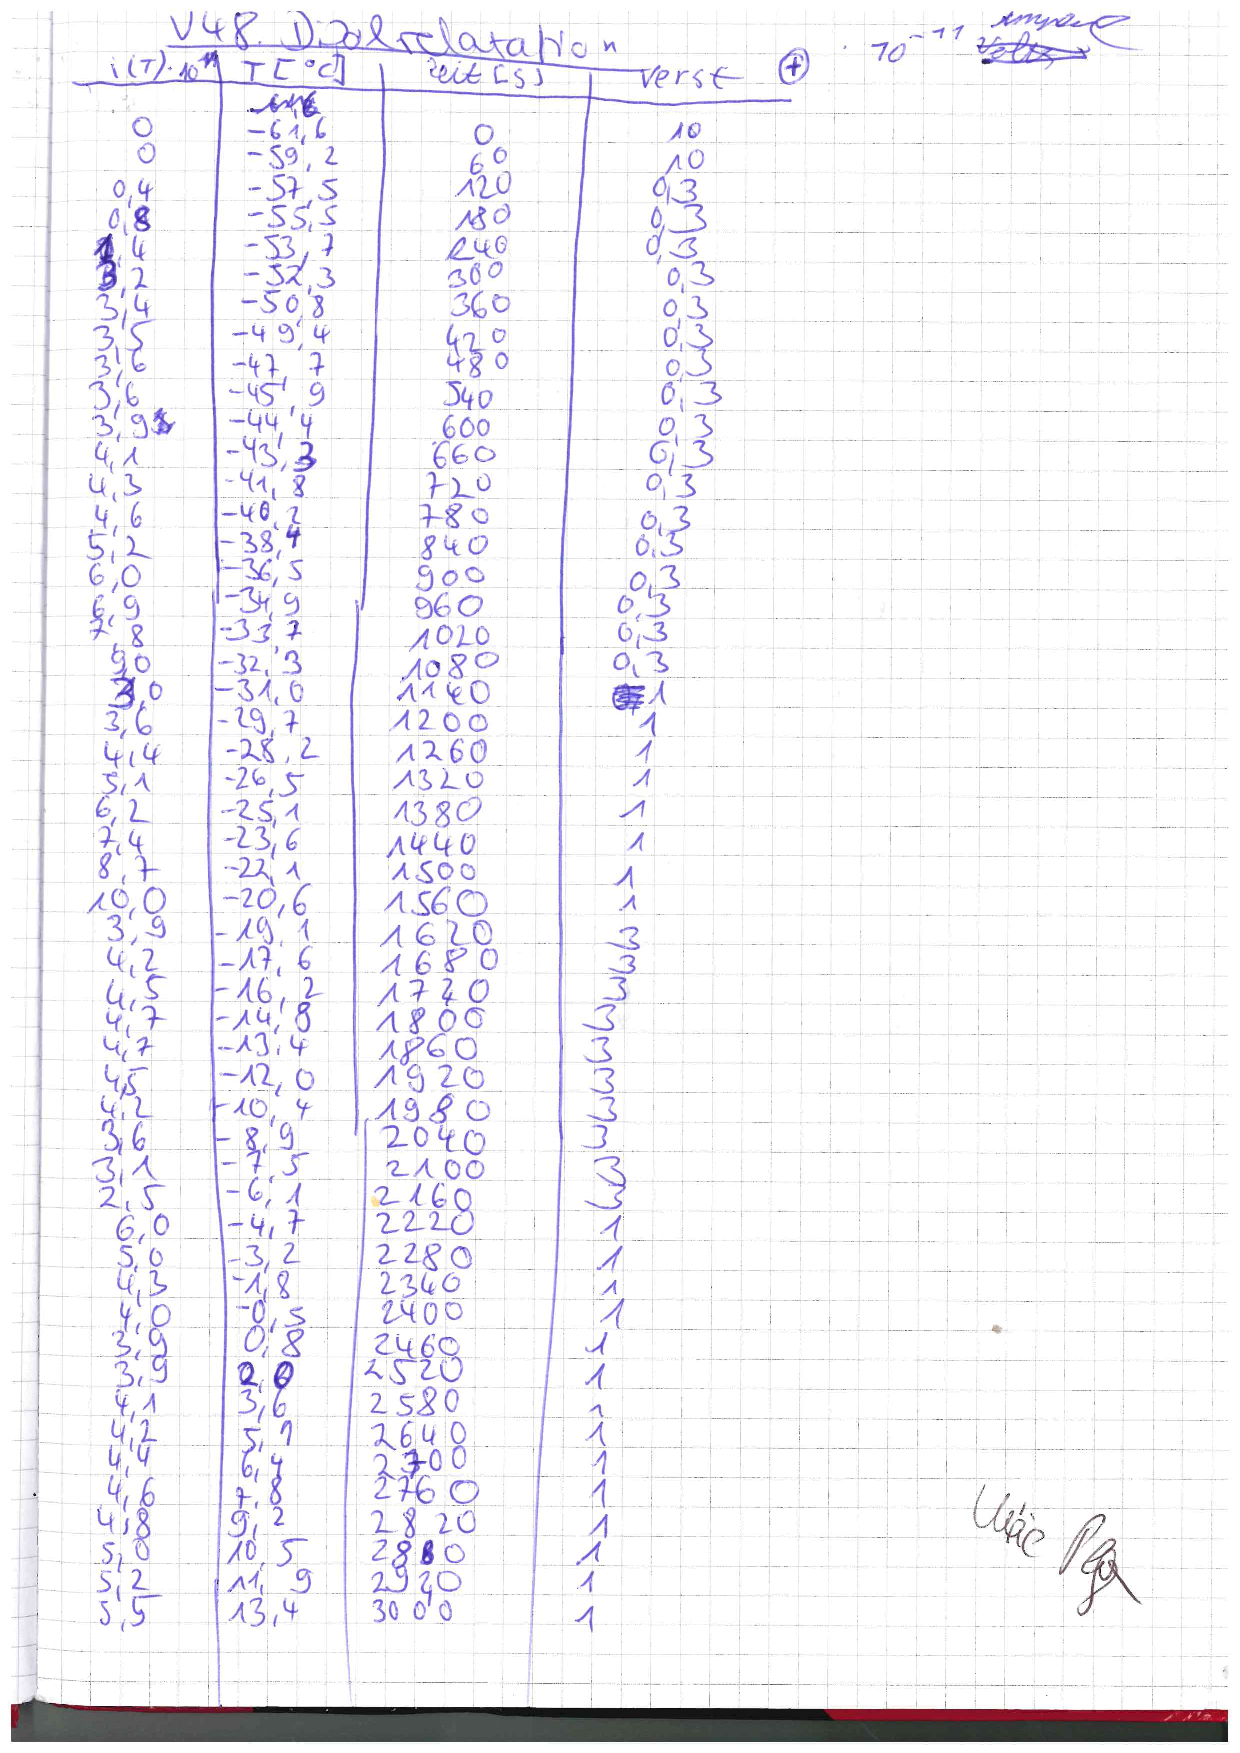
\includegraphics[angle=0, width = \textwidth]{V48-1.pdf}
\end{figure}
\begin{figure}
  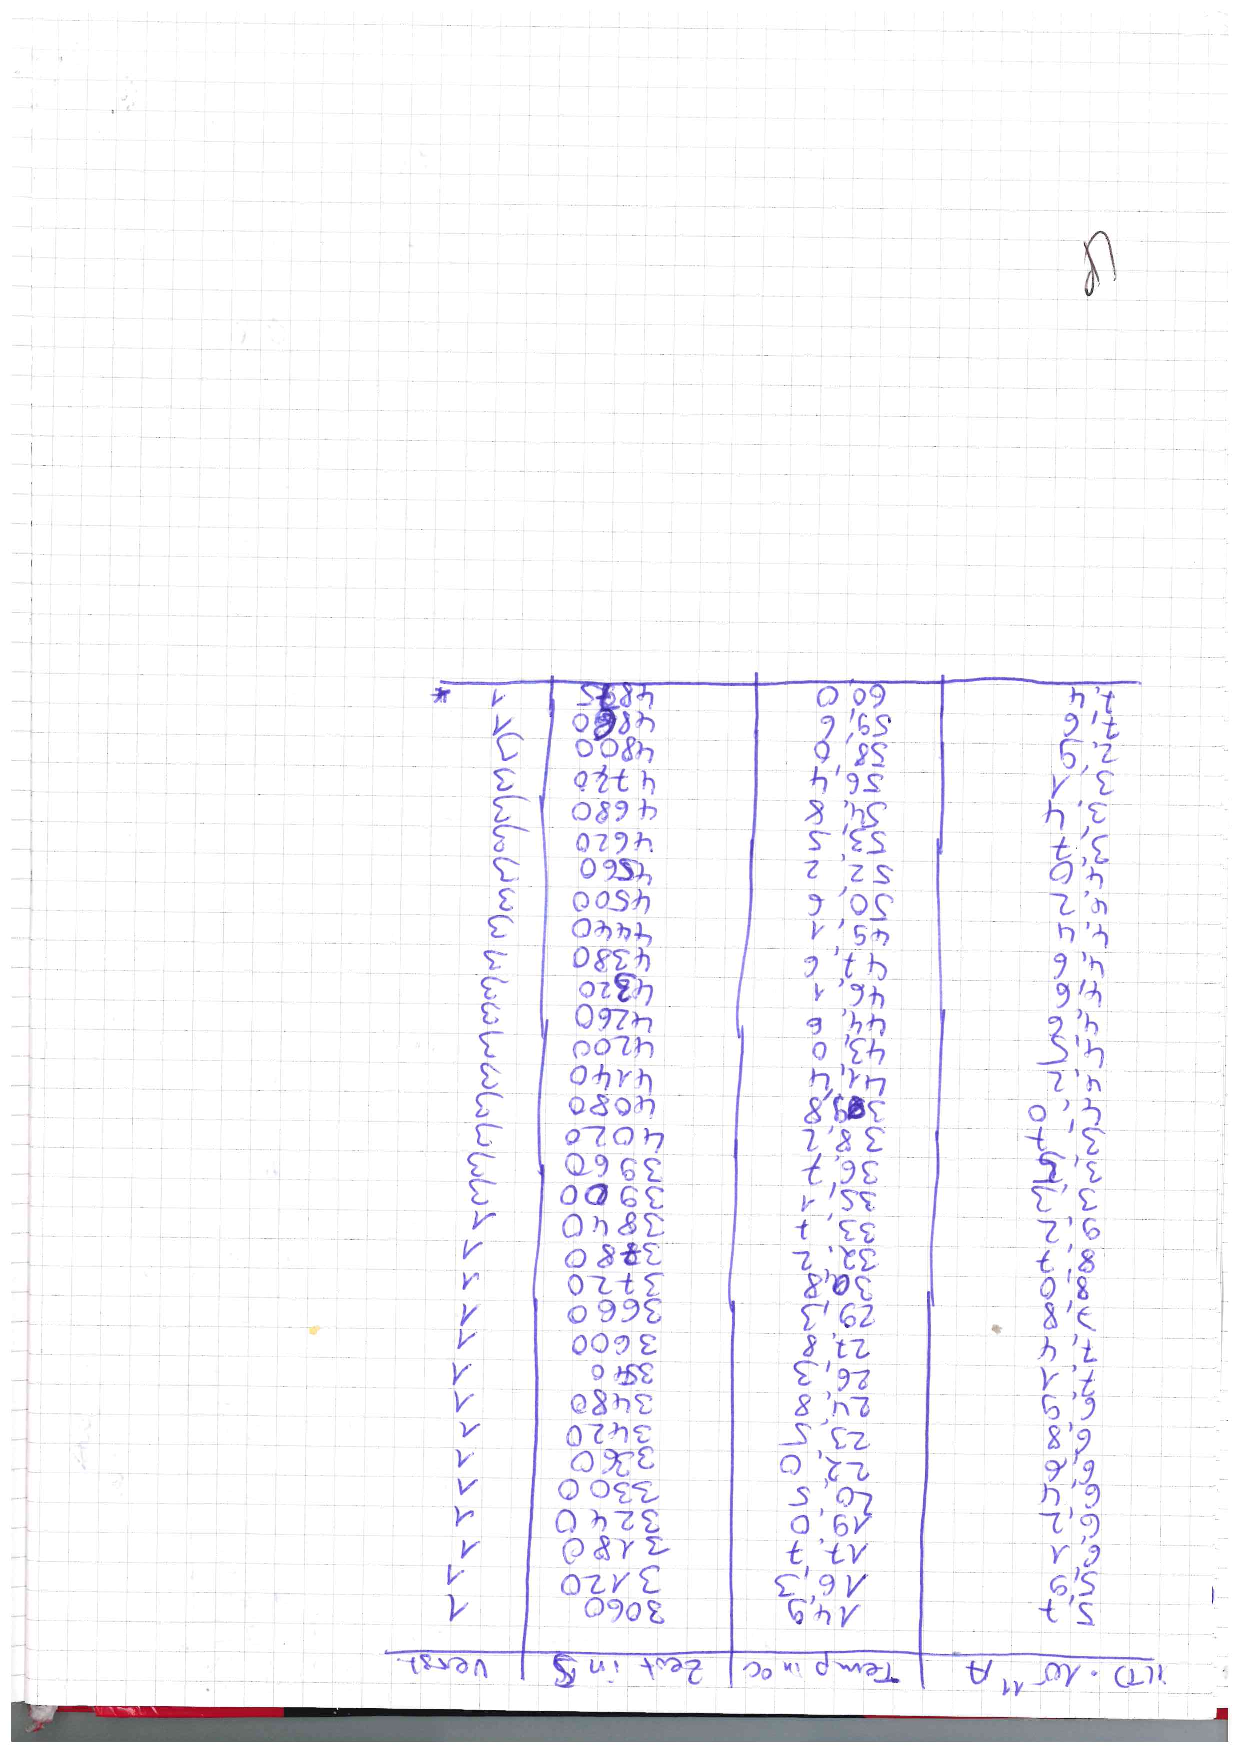
\includegraphics[angle=180, width = \textwidth]{V48-2.pdf}
\end{figure}
\begin{figure}
  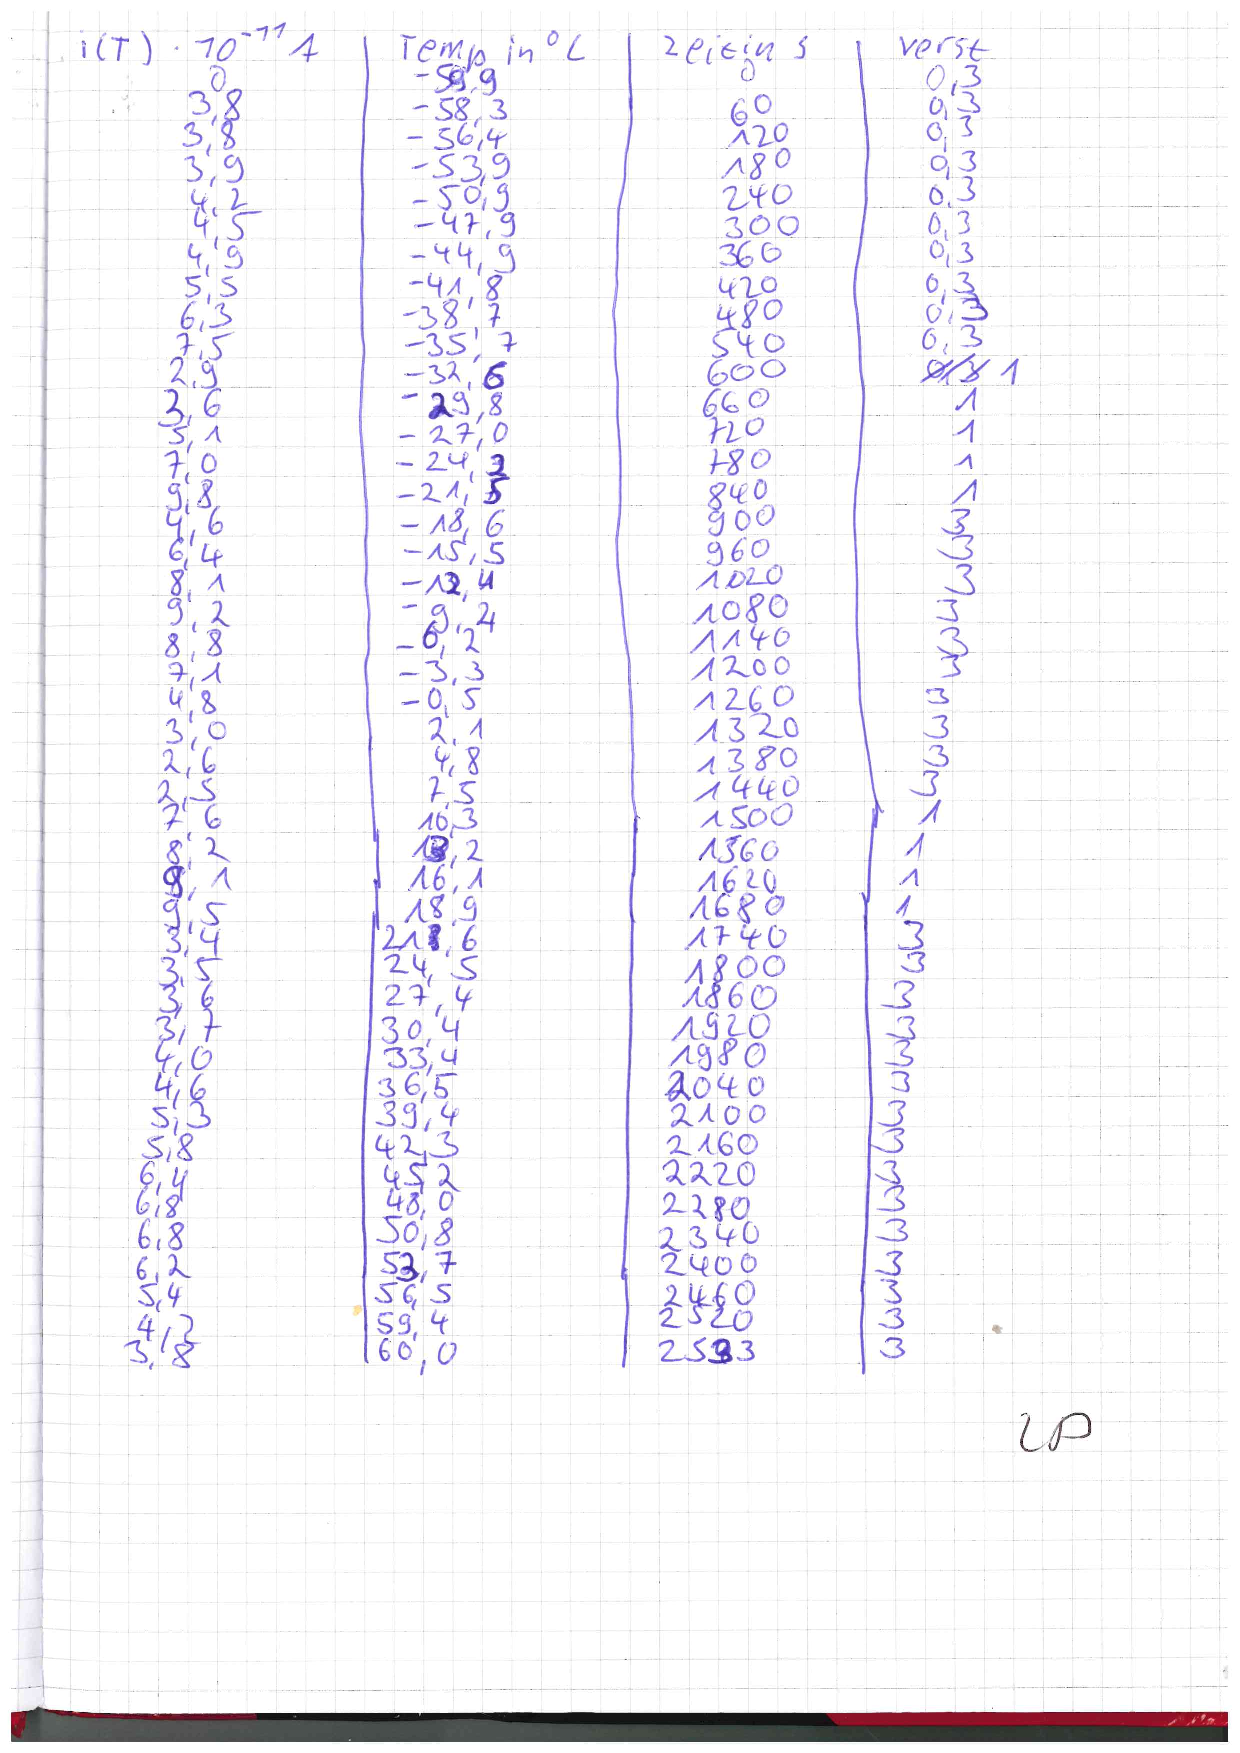
\includegraphics[angle=0, width = \textwidth]{V48-3.pdf}
\end{figure}
